\documentclass[english]{PaperTools/latex/lipics}
\graphicspath{{PaperTools/latex/}}
\usepackage{natbib}
\usepackage[utf8]{inputenc}
\usepackage{stmaryrd}
\usepackage{amssymb,amstext,amsmath}
\usepackage{mathtools}
\usepackage{mathpartir}
\usepackage{fancyref}
\usepackage{todonotes}
\newcommand{\Freflemname}{Lem.}
\newcommand{\freflemname}{Lem.}
\newcommand*{\fancyreflemlabelprefix}{lem}
\frefformat{vario}{\fancyreflemlabelprefix}{%
       \textnormal{\freflemname}\fancyrefdefaultspacing#1}
\Frefformat{vario}{\fancyreflemlabelprefix}{%
       \textnormal{\Freflemname}\fancyrefdefaultspacing#1}
%\newtheorem{lemma}{\Freflemname}

\newcommand{\Frefdefname}{Def.}
\newcommand{\frefdefname}{Def.}
\newcommand*{\fancyrefdeflabelprefix}{def}
\frefformat{vario}{\fancyrefdeflabelprefix}{%
       \textnormal{\frefdefname}\fancyrefdefaultspacing#1}

\newcommand{\Frefcorname}{Corollary}
\newcommand{\frefcorname}{Corollary}
\newcommand*{\fancyrefcorlabelprefix}{cor}
\frefformat{vario}{\fancyrefcorlabelprefix}{%
       \textnormal{\frefcorname}\fancyrefdefaultspacing#1}

\newcommand{\Frefthmname}{Th.}
\newcommand{\frefthmname}{Th.}
\newcommand*{\fancyrefthmlabelprefix}{thm}
\frefformat{vario}{\fancyrefthmlabelprefix}{%
       \textnormal{\frefthmname}\fancyrefdefaultspacing#1}
\Frefformat{vario}{\fancyrefthmlabelprefix}{%
       \textnormal{\Frefthmname}\fancyrefdefaultspacing#1}

\newcommand{\Frefpropname}{Prop.}
\newcommand{\frefpropname}{Prop.}
\newcommand*{\fancyrefproplabelprefix}{prop}
\frefformat{vario}{\fancyrefproplabelprefix}{%
       \textnormal{\frefpropname}\fancyrefdefaultspacing#1}
\Frefformat{vario}{\fancyrefproplabelprefix}{%
       \textnormal{\Frefpropname}\fancyrefdefaultspacing#1}


\frefformat{vario}{\fancyrefeqlabelprefix}{%
       \textnormal{(#1)}}

\renewcommand{\frefsecname}{Sec.}
\renewcommand{\freffigname}{Fig.}


\newcommand{\Frefexname}{Example}
\newcommand{\frefexname}{Example}
\newcommand*{\fancyrefexlabelprefix}{ex}
\frefformat{vario}{\fancyrefexlabelprefix}{%
       \textnormal{\frefexname}\fancyrefdefaultspacing#1}
\Frefformat{vario}{\fancyrefexlabelprefix}{%
       \textnormal{\Frefexname}\fancyrefdefaultspacing#1}

\frefformat{vario}{\fancyrefeqlabelprefix}{%
       \textnormal{(#1)}}

\usepackage{tikz}
\usetikzlibrary{arrows}

\newcommand\CC[4]{(#2,_{#1} #3)}
\newcommand\CP[3]{(#2,_{#1} #3)}
\newcommand\CTimes[2]{(#2) ×_{#1}}
\newcommand\SW[2]{\mathsf{SW}^{#1}_{#2}}
\newcommand\sw[2]{\mathsf{sw}^{#1}_{#2}}
\newcommand\dom{\mathsf{dom}}
\newcommand\param[1]{\!\cdot\!#1}
\newcommand\pvar[2]{{#1}^{(#2)}}
\newcommand\op[1]{∋_{#1}}
\newcommand\ip[3]{Σ^{#1} {#2}\,{#3}}
\newcommand\fp[3]{⟨#2 ,_{#1} #3⟩}
\newcommand\mor[2]{({#1}\,{#2})}
\newcommand\proj[2]{{#2}\,\mor{#1}0}
\newcommand\projp[2]{\proj{#1}{(#2)}}

\newcommand\comment[1]{}
\DeclareUnicodeCharacter{00A0}{~} %   NO-BREAK SPACE
\DeclareUnicodeCharacter{00A7}{\S} % §
\DeclareUnicodeCharacter{00AC}{\ensuremath{\neg}} % ¬
\DeclareUnicodeCharacter{00B0}{^{\circ}} % °
\DeclareUnicodeCharacter{00B1}{^1} 
\DeclareUnicodeCharacter{00B2}{^2} % ²
\DeclareUnicodeCharacter{00B7}{\ensuremath{\cdot}} % ·
\DeclareUnicodeCharacter{00B9}{\textsuperscript{l}} % ¹
\DeclareUnicodeCharacter{00D7}{\ensuremath{\times}} % × 
\DeclareUnicodeCharacter{00F7}{\ensuremath{\div}} % ÷
\DeclareUnicodeCharacter{02E1}{\ensuremath{{^l}}} % ˡ
\DeclareUnicodeCharacter{02B3}{\ensuremath{{^r}}} % ʳ
\DeclareUnicodeCharacter{0393}{\ensuremath{\Gamma}} % Γ
\DeclareUnicodeCharacter{0394}{\ensuremath{\Delta}} % Δ
\DeclareUnicodeCharacter{0397}{\ensuremath{\textrm{H}}} % Η
\DeclareUnicodeCharacter{0398}{\ensuremath{\Theta}} % Θ
\DeclareUnicodeCharacter{039B}{\ensuremath{\Lambda}} % Λ
\DeclareUnicodeCharacter{039E}{\ensuremath{\Xi}} % Ξ
\DeclareUnicodeCharacter{03A3}{\ensuremath{\Sigma}} % Σ
\DeclareUnicodeCharacter{03A6}{\ensuremath{\Phi}} % Φ
\DeclareUnicodeCharacter{03A8}{\ensuremath{\Psi}} % Ψ
\DeclareUnicodeCharacter{03A9}{\ensuremath{\Omega}} % Ω
\DeclareUnicodeCharacter{03B1}{\ensuremath{\mathnormal{\alpha}}} % α
\DeclareUnicodeCharacter{03B2}{\ensuremath{\beta}} % β
\DeclareUnicodeCharacter{03B3}{\ensuremath{\mathnormal{\gamma}}} % γ
\DeclareUnicodeCharacter{03B4}{\ensuremath{\mathnormal{\delta}}} % δ
\DeclareUnicodeCharacter{03B5}{\ensuremath{\mathnormal{\varepsilon}}} % ε
\DeclareUnicodeCharacter{03B6}{\ensuremath{\mathnormal{\zeta}}} % ζ
\DeclareUnicodeCharacter{03B7}{\ensuremath{\mathnormal{\eta}}} % η
\DeclareUnicodeCharacter{03B8}{\ensuremath{\mathnormal{\theta}}} % θ
\DeclareUnicodeCharacter{03B9}{\ensuremath{\mathnormal{\iota}}} % ι
\DeclareUnicodeCharacter{03BA}{\ensuremath{\mathnormal{\kappa}}} % κ
\DeclareUnicodeCharacter{03BB}{\ensuremath{\mathnormal{\lambda}}} % λ
\DeclareUnicodeCharacter{03BC}{\ensuremath{\mathnormal{\mu}}} % μ
\DeclareUnicodeCharacter{03BD}{\ensuremath{\mathnormal{\mu}}} % ν
\DeclareUnicodeCharacter{03BE}{\ensuremath{\mathnormal{\xi}}} % ξ
\DeclareUnicodeCharacter{03C0}{\ensuremath{\mathnormal{\pi}}} % π
\DeclareUnicodeCharacter{03C1}{\ensuremath{\mathnormal{\rho}}} % ρ
\DeclareUnicodeCharacter{03C3}{\ensuremath{\mathnormal{\sigma}}} % σ
\DeclareUnicodeCharacter{03C4}{\ensuremath{\mathnormal{\tau}}} % τ
\DeclareUnicodeCharacter{03C6}{\ensuremath{\mathnormal{\varphi}}} % φ
\DeclareUnicodeCharacter{03D5}{\ensuremath{\mathnormal{\phi}}} % ϕ
\DeclareUnicodeCharacter{03C7}{\ensuremath{\mathnormal{\chi}}} % χ
\DeclareUnicodeCharacter{03C8}{\ensuremath{\mathnormal{\psi}}} % ψ
\DeclareUnicodeCharacter{03C9}{\ensuremath{\mathnormal{\omega}}} % ω 
\DeclareUnicodeCharacter{03F5}{\ensuremath{\mathnormal{\epsilon}}} % ϵ
\DeclareUnicodeCharacter{1D62}{_i} % ᵢ
\DeclareUnicodeCharacter{10627}{\ensuremath{\lbana}} 
\DeclareUnicodeCharacter{10628}{\ensuremath{\rbana}} 
\DeclareUnicodeCharacter{2026}{\ensuremath{\ldots}}
\DeclareUnicodeCharacter{202F}{{\,}}
\DeclareUnicodeCharacter{2080}{\ensuremath{_0}} % ₀
\DeclareUnicodeCharacter{2081}{\ensuremath{_1}}
\DeclareUnicodeCharacter{2082}{\ensuremath{_2}}
\DeclareUnicodeCharacter{2083}{\ensuremath{_3}}
\DeclareUnicodeCharacter{2084}{\ensuremath{_4}}
\DeclareUnicodeCharacter{2085}{\ensuremath{_5}}
\DeclareUnicodeCharacter{2086}{\ensuremath{_6}}
\DeclareUnicodeCharacter{2087}{\ensuremath{_7}}
\DeclareUnicodeCharacter{2088}{\ensuremath{_8}}
\DeclareUnicodeCharacter{2089}{\ensuremath{_9}}
\DeclareUnicodeCharacter{2115}{\mathbb{N}}
\DeclareUnicodeCharacter{214B}{\ensuremath{\parr}}
\DeclareUnicodeCharacter{2190}{\ensuremath{\leftarrow}} % ← 
\DeclareUnicodeCharacter{2191}{\ensuremath{\uparrow}} % ↑
\DeclareUnicodeCharacter{2192}{\ensuremath{\rightarrow}} % →
\DeclareUnicodeCharacter{2194}{\ensuremath{\leftrightarrow}} % ↔
\DeclareUnicodeCharacter{2196}{\nwarrow} % ↖
\DeclareUnicodeCharacter{2197}{\nearrow} % ↗
\DeclareUnicodeCharacter{219D}{\ensuremath{\leadsto}} % ↝
\DeclareUnicodeCharacter{21A6}{\ensuremath{\mapsto}} % ↦ 
\DeclareUnicodeCharacter{21C6}{\ensuremath{\leftrightarrows}} % ⇆
\DeclareUnicodeCharacter{21D0}{\ensuremath{\Leftarrow}} % ⇐
\DeclareUnicodeCharacter{21D2}{\ensuremath{\Rightarrow}} % ⇒ 
\DeclareUnicodeCharacter{21D4}{\ensuremath{\Leftrightarrow}} % ⇔
\DeclareUnicodeCharacter{2200}{\ensuremath{\forall}} % ∀
\DeclareUnicodeCharacter{2203}{\ensuremath{\exists}} % ∃
\DeclareUnicodeCharacter{2205}{\ensuremath{\varnothing}} % ∅
\DeclareUnicodeCharacter{2208}{\ensuremath{\in}} % ∈
\DeclareUnicodeCharacter{2209}{\ensuremath{\not\in}} % ∉
\DeclareUnicodeCharacter{220B}{\ensuremath{\ni}}
\DeclareUnicodeCharacter{220E}{\ensuremath{\qed}} % ∎ % Alternatively use \blacksquare
\DeclareUnicodeCharacter{2211}{\sum}% ∑
\DeclareUnicodeCharacter{2215}{\mathbb{N}} % ℕ
\DeclareUnicodeCharacter{2217}{\ensuremath{\ast}} % ∗
\DeclareUnicodeCharacter{2218}{\ensuremath{\circ}} % ∘
\DeclareUnicodeCharacter{2219}{\ensuremath{\bullet}} % ∙ 
\DeclareUnicodeCharacter{221E}{\ensuremath{\infty}} % ∞
\DeclareUnicodeCharacter{2223}{\ensuremath{\mid}} % ∣
\DeclareUnicodeCharacter{2227}{\wedge}% ∧
\DeclareUnicodeCharacter{2228}{\vee}% ∨
\DeclareUnicodeCharacter{2229}{\ensuremath{\cap}} % ∩
\DeclareUnicodeCharacter{222A}{\ensuremath{\cup}} % ∪
\DeclareUnicodeCharacter{2237}{::} % ∷
\DeclareUnicodeCharacter{223C}{\ensuremath{\sim}} % ∼
\DeclareUnicodeCharacter{2243}{\ensuremath{\simeq}} % ≃
\DeclareUnicodeCharacter{2245}{\ensuremath{\cong}} % ≅ 
\DeclareUnicodeCharacter{2248}{\ensuremath{\approx}} % ≈
\DeclareUnicodeCharacter{225C}{\ensuremath{\stackrel{\scriptscriptstyle {\triangle}}{=}}} % ≜
\DeclareUnicodeCharacter{225F}{\ensuremath{\stackrel{\scriptscriptstyle ?}{=}}} % ≟
\DeclareUnicodeCharacter{2260}{\neq}% ≠
\DeclareUnicodeCharacter{2261}{\equiv}% ≡
\DeclareUnicodeCharacter{2264}{\ensuremath{\le}} % ≤
\DeclareUnicodeCharacter{2265}{\ensuremath{\ge}} % ≥
\DeclareUnicodeCharacter{2282}{\ensuremath{\subset}} % ⊂
\DeclareUnicodeCharacter{2283}{\ensuremath{\supset}} % ⊃ 
\DeclareUnicodeCharacter{2286}{\ensuremath{\subseteq}} % ⊆ 
\DeclareUnicodeCharacter{2287}{\ensuremath{\supseteq}} % ⊇
\DeclareUnicodeCharacter{2293}{\ensuremath{\sqcup}} % ⊓
\DeclareUnicodeCharacter{2293}{\sqcap} % ⊓
\DeclareUnicodeCharacter{2294}{\sqcup} % ⊔
\DeclareUnicodeCharacter{2295}{\ensuremath{\oplus}} % ⊕
\DeclareUnicodeCharacter{2297}{\ensuremath{\otimes}} % ⊗
\DeclareUnicodeCharacter{22A2}{\ensuremath{\vdash}}
\DeclareUnicodeCharacter{22A4}{\ensuremath{\top}} % ⊤
\DeclareUnicodeCharacter{22A5}{\ensuremath{\bot}} % ⊥
\DeclareUnicodeCharacter{22A7}{\models} % ⊧ 
\DeclareUnicodeCharacter{22A8}{\models} % ⊨
\DeclareUnicodeCharacter{22A9}{\Vdash} % ⊩
\DeclareUnicodeCharacter{22B8}{\ensuremath{\multimap}} % ⊸
\DeclareUnicodeCharacter{22C4}{\diamond} % ⋄
\DeclareUnicodeCharacter{22C6}{\ensuremath{\star}}
\DeclareUnicodeCharacter{22EE}{\ensuremath{\vdots}} % ⋮
\DeclareUnicodeCharacter{22EF}{\ensuremath{\cdots}} % ⋯
\DeclareUnicodeCharacter{2308}{\ensuremath{\lceil}}
\DeclareUnicodeCharacter{2309}{\ensuremath{\rceil}}
\DeclareUnicodeCharacter{230A}{\ensuremath{\lfloor}}
\DeclareUnicodeCharacter{230B}{\ensuremath{\rfloor}}
\DeclareUnicodeCharacter{25A1}{\ensuremath{\square}} % □
\DeclareUnicodeCharacter{25AF}{\mathop{\talloblong}} % ▯
\DeclareUnicodeCharacter{25C7}{\diamond} % ◇
\DeclareUnicodeCharacter{2605}{\ensuremath{\star}}   % ★
\DeclareUnicodeCharacter{2713}{\ensuremath{\checkmark}} % ✓
\DeclareUnicodeCharacter{27C2}{\ensuremath{^\bot}} % PERPENDICULAR ⟂
\DeclareUnicodeCharacter{27E6}{\ensuremath{\llbracket}} % ⟦
\DeclareUnicodeCharacter{27E7}{\ensuremath{\rrbracket}} % ⟧
\DeclareUnicodeCharacter{27E8}{\ensuremath{\langle}} % ⟨
\DeclareUnicodeCharacter{27E9}{\ensuremath{\rangle}} % ⟩
\DeclareUnicodeCharacter{27F6}{{\longrightarrow}} % ⟶
\DeclareUnicodeCharacter{27F7}{{\longleftrightarrow}} % ⟷
\DeclareUnicodeCharacter{2A04}{\mathop{\dot{\cup}}} % ⨄
\DeclareUnicodeCharacter{2AFE}{\mathop{\talloblong}} % ⫾

% \DeclareUnicodeCharacter{8499}{\mathcal{M}} 
% \DeclareUnicodeCharacter{8718}{\ensuremath{\blacksquare}}
% \DeclareUnicodeCharacter{8797}{\mathrel{\mathop:}=}
% \DeclareUnicodeCharacter{9657}{\ensuremath{\triangleright}}
% \DeclareUnicodeCharacter{9667}{\triangleright{}}
% \DeclareUnicodeCharacter{9669}{\ensuremath{\triangleleft}}


\def\pI{\ensuremath{\mathbf{pI}}}
\def\fresh#1{\mathsf{fresh}(#1)}
\def\Hom#1#2{\mathbf{Hom}(#1,#2)}
\def\ie{\textit{i.e.}}
\def\app#1#2{\mathsf{app}(#1,#2)}
\def\El#1{\mathrm{El}(#1)}

\title{A presheaf model of parametric type-theory}

\author{}
\date{\today}

\begin{document}
\maketitle

\begin{abstract}
  We propose a new type-theory with internalized
  parametricity. Compared to previous similar proposals, this version
  comes with a denotational semantics which is a refinement of the
  standard presheaf semantics of dependent type theory. Further, this
  presheaf semantics is a refinement of the one used to interpret
  nominal sets with restriction.  This calculus is a candidate for the
  core of a proof assistant with internalized parametricity.
\end{abstract}

\section{Introduction}
In lambda-calculi, every type can be interpreted as a predicate, which
its inhabitants are guaranteed to satisfy.
%
A simple example is that if a function $f$ has type $(A : U) → U → U$ ---
the type of the polymorphic identity --- then the following
proposition holds:
%
\[
  (A : U) → (P : A → U) → (x : A) → P x → P (f A x)
\]
%
(which implies that $f$ must return exactly its argument).
The above result, \emph{abstraction}, has proved useful for reasoning
about functional programs \citep{wadler_theorems_1989}. It also has deep
theoretical implications: for example, the induction principle over Church numerals
can be deduced from it \citep{wadler_girardreynolds_2007}.


The abstraction theorem is an invention of
\citet{reynolds_types_1983}, which he used to give formal meaning to
polymorphism in the λ-calculus. He does so by a model construction
where types are interpreted as predicates and functions are interpreted
by predicate-preserving functions.

In this paper, we propose an extension of Reynolds' model, where a
type is interpreted as a hypercube of sets, predicates, relations,
relations between relations and so on. Our model
supports the interpretation dependent type-theories, and of
parametricity itself (parametricity is parametric).  We take advantage of this
closure property by intergrating parametricity into the syntax of the
type-theory being interpreted.  This means that the user of the logic
can prove any parametricity result directly in the logic, rather than
having to resort to an external semantic justification.

Our technical contributions are as follows:
\begin{itemize}
\item We propose a novel type-theory (\fref{sec:syntax}), and show
  that it internalises parametricity (\fref{sec:parametricity}).
  % In particular, we show that the calculus internalizes parametricity. 
  % in \fref{sec:abstraction}. \comment{Much of this is now in the appendix...}
\item We provide a presheaf model for this type-theory. \todo{what+refs}
\end{itemize}

\section{Syntax}
\label{sec:syntax}
In the following section we define the syntax and typing-rules of our
parametric type-theory, as well as the equality judgement.

We assume a set of symbols, called \emph{colors}.
The metasyntactic variables $i,j,\ldots$ range over colours, while
$I,J,…$ range over finite sets of colours.

Compared to type-theory, the main innovation of the type-theory
presented here is that terms may depend on (a finite number of)
colours.
\begin{definition}[Syntax of terms and contexts]
  \begin{align*}
    t,u,A,B & \coloneqq x & \text {variable} \\
            & \mid U & \text{universe} \\ 
            & \mid |A| & \text{code} \\ 
            & \mid El(A) & \text{decode} \\ 
            & \mid λx:A. t & \text{abstraction} \\
            & \mid t u & \text{application} \\ 
            & \mid (x:A) → B & \text{product} \\
            & \mid \CP i t u & \text{colored pair} \\
            & \mid \CTimes i {x:A} B  & \text{colored type pair} \\
            & \mid \fp i t u & \text{colored function pair}\\
            & \mid A \op i u & \text{parametricity type} \\
            & \mid t \param i & \text{parametricity proof} \\
    \Gamma,\Delta & \coloneqq () \mid \Gamma,x:A
  \end{align*}
\end{definition}

\begin{itemize}
\item Each color $i$ may be erased from a term $a$ to obtain a realiser, written $\proj i a$ (detailed in \fref{def:color-subst}).
\item the type $A \op i u$, which expresses that $u$ satisfies the
  parametricity predicate associated with the type $A$ on color $i$.
\item the term $a \param i$, which yields a proof of $A \op i \proj i a$.
\item the forms $\CP i t u$, $\CTimes i A B$ and $\fp i t u$ allow to
  locally associate parametricity proofs with a given realizer.
\end{itemize}



\begin{definition}[Typing judgements — à la Tarski]
We mutually define three judgments:
\begin{itemize}
\item $Γ⊢_I$ (Is the context $Γ$ is well-formed, assuming the color set $I$?).
\item $Γ⊢_I A$  (Is the type $A$ well-formed in $Γ$ and assuming the color set $I$?)
\item $Γ⊢_I a : A$  (Does the term $a$ have type $A$ in the context $Γ$ and assuming the color set $I$?)
\end{itemize}

\fbox{$Γ⊢_I$}
  \begin{mathpar}
    \inferrule[Empty]{~}{() ⊢_I }

    \inferrule[NewVar]{Γ⊢_I \\ Γ ⊢_I A }{ Γ,x:A ⊢_I }

  \end{mathpar}
 
\fbox{$Γ⊢_I A$}
 \begin{mathpar}

    \inferrule[Universe]{}{Γ ⊢_I U}

    \inferrule[Decode]{Γ ⊢_I A : U}{Γ ⊢_I \El{A}}

    \\
    \inferrule[Pi]{Γ ⊢_I A \\ Γ,x:A ⊢_I B}{Γ ⊢_I (x:A) → B}

    \inferrule[Out]{Γ ⊢_{I,i} T \\ Γ ⊢_I a : \proj i T}{Γ ⊢_I T \op i  a}

    \inferrule[In-Pred]{Γ ⊢_{I} A \\ Γ,x:A ⊢_{I} B}{Γ ⊢_{I,i} \CTimes i {x:A} B}
 \end{mathpar}

\fbox{$Γ⊢_I a : A$}
  \begin{mathpar}
    \inferrule[Conv]{Γ ⊢_I t:A \\ A = B}{Γ ⊢_I t : B}

    \inferrule[Var]{Γ ⊢_I \\ x : A ∈ Γ}{Γ ⊢_I x : A}

    \inferrule[Code]{Γ ⊢_I A }{Γ ⊢_I |A| : U}

    \\\inferrule[Lam]{Γ,x:A ⊢_I B}{Γ ⊢_I λx:A.b : (x:A) → B}
 
    \inferrule[App]{Γ ⊢_I t : (x:A) → B[x] \\ Γ ⊢_I u : A}{Γ ⊢_I t u: B[u]}

    \\\inferrule[In-Abs]{Γ ⊢_I a : \proj i T \\Γ ⊢_I p : T \op i a}{Γ ⊢_{I,i} \CP i a p : T}

    \inferrule[In-Fun]
        {Γ ⊢_I f : \projp i {(x:A) → P x}\\\\
        Γ ⊢_I g : (x:\proj i A) → (x':A \op i x) → P \CP i x {x'} \op i f x}{Γ ⊢_{I,i} \fp i f g : (x:A) → P x}

    \inferrule[Color-elim]{Γ ⊢_{I,i} a : T}{Γ ⊢_I a \param i : T \op i {\proj i a}}


  \end{mathpar}
\end{definition}

The parametricity constructions ($·$ and $∋$) act like color
binders (they bring colors into scope), while the pairing constructs
remove colors from scope.
The equality relation used in the {\sc Conv} rule is detailed below in \fref{def:conversion}.

\begin{definition}[$I$-term]
\todo{TODO}
\end{definition}
\begin{definition}[$\fresh I$]
\todo{TODO}
\end{definition}

% 'Morphism' means something only in the context of a category; hence Morphism application ==> Color substitution
\begin{definition}[Color substitution]~
  \label{def:color-subst}
  We consider partial injections $f : I → J$ and for any $I$-term $a$,
  we define the $J$-term $af$ by structural induction on $a$.
  We note $(i\,0) : I,i → I$ the partial identity.
\begin{align*}
  x f & = x \\
  U f & = U \\
  (λ(x:A).t) f &= λ(x:Af).tf \\
  (t\,u) f &= (tf) \, (uf) \\
  ((x:A)→B) f &= (x:Af)→(Bf) \\
  \CP {i} a p f &= \CP {j} {ag} {pg}
    & \text{if $fi = j$, $g : I→J_{\{j\}}$ such that $(i\,0)g = f(j\,0) : I,i → J_{\{j\}}$} \\
                &= ag
    & \text{if $∃g : I→J$ such that $f = (i\,0)g : I,i → J$} \\
  (\CTimes {i} A B) f &= \CTimes {j} {(Ag)} {(Bg)}
    & \text{if $fi = j$, $g : I→J_{\{j\}}$ such that $(i\,0)g = f(j\,0) : I,i → J_{\{j\}}$} \\
                &= Ag
    & \text{if $∃g : I→J$ such that $f = (i\,0)g : I,i → J$} \\
  \fp {i} u v f &= \fp {j} {ug} {vg}
    & \text{if $fi = j$, $g : I→J_{\{j\}}$ such that $(i\,0)g = f(j\,0) : I,i → J_{\{j\}}$} \\
                &= ug
    & \text{if $∃g : I→J$ such that $f = (i\,0)g : I,i → J$} \\
  A \op {i} a &= (Ag) \op {j} (af)
    & \text{where $j = \fresh J$ and $g:I,i → J,j$ satisfies $(i\,0)f = g(j\,0)$} \\
  (a · i) f &= (ag) · j
    & \text{where $j = \fresh J$ and $g:I,i → J,j$ satisfies $(i\,0)f = g(j\,0)$}
\end{align*}
  (We remark that for any $f : I,i → J,j$ with $fi=j$, there is a
  unique $g : I → J$ such that $(i\,0)g = f(j\,0) : I,i → J$;
  and that for any $f : I,i → J$ which is not defined on $i$, there is
  a unique $g : I → J$ such that $(i\,0)g = f$.)

  We have $a1 = a$ and $(af)g = a(fg)$ for any $g : J → K$.
  Furthermore, if $Γ ⊢_I a : A$ then $Γ f ⊢_J af : Af$ (proof by
  induction on the typing judgement).
\end{definition}

\comment{
\begin{definition}[Normal forms and neutral terms]~
  \begin{align*}
    \mathsf{Nf} ∋ u,v,A,B & \coloneqq
      U \mid λx:A. t \mid (x:A) → B \\
      & \mid \CP i u v \mid \fp i u v \\
      & \mid {(\CTimes {i₀} A B)} \op {i₁} {u_1 \cdots} \op {i_n} {u_n} &\quad \text{($i₀ \prec i₁ \prec \ldots \prec i_n$)} \\
      & \mid s \param {i₀} \cdots \param {i_{n-1}}                  &\quad \text{($i₀ \prec   < \ldots \prec i_{n-1}$)}
    \\
    \mathsf{Ne} ∋ s & \coloneqq x \mid s \, u
  \end{align*}
\end{definition}
}

\begin{definition}[Conversion]~
\label{def:conversion}
The convertibity of types (noted $=$) as an untyped relation, defined inductively by the following rules:
\begin{mathpar}
  \inferrule[Pair-App]{}{{\fp i f g} \, a      = (f\,{\proj i a} ,_i g\,{\proj i a}\,{(a \param i)})}
\and
  \inferrule[Pair-Param]{}{{(a,_i p)}\param i   = p}
\and
  \inferrule[Pair-Pred]{}{{(\CTimes i {x:A} B[x])} \op i a = B[a]}
\and
    \inferrule{}{\El{|A|} = A}
\and
    \inferrule{}{|\El{A}| = A}
\and
    \inferrule[β]{}{(λx:A. u[x]) t = u[t]}
\and
    \inferrule[η]{t x = u} {t = λ x:A.u}
    \and
    \inferrule[Surj-Param]{\proj i t = a \\ t \param i = p} {t = \CP i a p }
    \and
    \inferrule[Surj-Fun]{\proj i t = f \\ (t \CP i x y) \param i = g x y} {t = \fp i f g }
    \and
    \inferrule[Surj-Typ]{\proj i T = A \\ T \op i x = B} {T = \CTimes i {x:A} B }
    \and
    \inferrule[Refl]{~}{a = a}
    \and
    \inferrule[Sym]{a = b}{b = a}
    \and
    \inferrule[Trans]{a = b \\ b = c}{a = c}
  \end{mathpar}
Additionally, all congruences yield convertibity rules.
\end{definition}


\begin{corollary}~
  \label{cor:equalities}
  \begin{itemize}
  \item $a = \CP i {\proj i a} {a \param i}$
  \item $T = \CTimes i {x:\proj i T} {(T \op i x)}$
  \item $f = \fp i {\proj i f} {λx x'. (f \CP i x {x'}) \param i}$
  \end{itemize}
\end{corollary}

\section{Parametricity}
\label{sec:parametricity}

Contrary to type-theories with internalized parametricity
\citep{bernardy_computational_2012,
  bernardy_type-theory_2013}, the system presented here lacks equalities
which allow to compute parametricity types. Expressed in our syntax, those equalites are:
$$U \op i A = A → U$$
and
$$((x:A) → B[x]) \op i f = (x:A) → (x' : A \op i x) → B[\CP i x {x'}] \op i (f x).$$

% \subsubsection{Isomorphisms}
Instead, we provide the above relationships as isomorphisms. The
existence of these isomorphisms ensure that all parametricity theorems
hold in the present system.

We say that $A$ is isomorphic to $B$ iff.
\begin{enumerate}
  \item There exist $f : A → B$
  \item There exist $g : B → A$
  \item For any $x$, $f (g x) = x$
  \item For any $x$, $g (f x) = x$
\end{enumerate}

\begin{theorem}
\label{thm:iso-univ}
$U \op i A$ is isomorphic to $A → U$.
\end{theorem}
\begin{proof}~
  \begin{enumerate}
  \item
    $\begin{array}[t]{l@{\,}l@{\,}l}
      f : (&Q : U \op i A) → &A → U \\ 
      f & Q &x = \CP i A Q \op i x
    \end{array}$
  \item
    $\begin{array}[t]{r@{\,}l}
      g &: (P : A → U) → U \op i A\\
      g &P = (\CTimes i {x:A} (P x)) \param i
    \end{array}$
  \item $\CP i A {(\CTimes i {y:A} (P y)) \param i} \op i x = (\CTimes i {y:A} (P x) \op i x = P x$ By eta-contraction we get the desired result.
  \item $(\CTimes i {x:A} {\CP i A Q \op i x}).i = Q$ if $\CTimes i {x:A} {\CP i A Q \op i x} = \CP i A Q$. We then use equality for $×_i$. The first components are obviously equal. For the second components we are left with $\CP i A Q \op i x = \CP i A Q \op i x$, which holds by reflexivity.
  \end{enumerate}
\end{proof}

\begin{theorem}
\label{thm:iso-fun}
$((x:A) → B[x]) \op i f$ is isomorphic to $(x:A) → (x' : A \op i x) → B[\CP i x {x'}] \op i (f x)$.
\end{theorem}
\begin{proof}~
  \begin{enumerate}
  \item $\begin{array}[t]{r@{\,}l}
      f &: (q : ((x:A) → B[x]) \op i f) → (x:A) → (x' : A \op i x) → B[\CP i x {x'}] \op i (f x)\\
      f &q x x' = (\CP i f q \CP i x {x'}) \param i
    \end{array}$
  \item $\begin{array}[t]{r@{\,}l}
      g &: ((x:A) → (x' : A \op i x) → B[\CP i x {x'}] \op i (f x)) →  ((x:A) → B[x]) \op i f\\
      g & p= \fp i f p \param i
    \end{array}$
  \item $(\CP i f {\fp i f p \param i} \CP i x x') \param i = ({\fp i
      f p} \CP i x {x'}) \param i = \CP i {f x} {p x x'} \param i = p
    x x' $
  \item $\fp i f {λx x'. (\CP i f q \CP i x {x'}) \param i} \param i$
    iff $\fp i f {λx x'. (\CP i f q \CP i x {x'}) \param i} = \CP i f
    q$, which is true by the equality rule for function pairing.
  \end{enumerate}
\end{proof}

In practice, when carrying out parametricity proofs, many of the steps
of the above isomorphisms cancel each other and one obtains a simpler
proof. This property is illustrated by the following example:
parametricity for Church-encoded natural numbers.
\begin{example}
Let $N = ∀X. X → (X → X) → X$.
Proving (unary) parametricity for $N$ means that, assuming
\begin{itemize}
\item $f : N$
\item $A : U$
\item $P : A → U$
\item $z : A$
\item $z' : P z$
\item $s : A → A$
\item $s' : (x:A) → P x → P (s x)$
\end{itemize}
we can prove $P (f A z s)$.

Indeed, a proof term is the following:
%
\[
(f (\CTimes i {x:A} (P x)) \CP i z {z'} \fp i s {s'}) \param i
\]
\end{example}

\subsection{Iterating Parametricity}
In our system, one can use parametricity generically as follows:
\begin{align*}
p &: (A:U) → (x:A) → A \op i x\\
p x &= x\param i
\end{align*}
We have already seen that $A \op i $ corresponds to the parametricity
predicate for type $A$. We can iterate this operator to construct
relations. That is, given
\begin{align*}
  x & :A \\
  y & : A \op i x\\
  z & : A \op i x
\end{align*}
Then the type $A \op i \CP j x y \op j z$ is well formed ($∋$ is left
associative), and can be understood as a relation
between the parametricity proofs $y$ and $z$. We have the following results on those relation.
\begin{theorem}
If the type $A$ does not depend on either $i$ or $j$, the relation $λy z. A \op i \CP j x y \op j z$ is symmetric.
\end{theorem}
\begin{proof}
  We first construct the proof term:
  \begin{align*}
    s & : (x:A) → (y : A \op i x) → (z : A \op i x) → (w : A \op i \CP j x y \op j z) → A \op j \CP i x z \op i y \\
    s & x y z w = \CP i {\CP j x y}{\CP j z w} \param j \param i
  \end{align*}
  And, by α-equivalence, $A \op j \CP i x z \op i y = A \op i \CP j x z \op j y$.
\end{proof}
\begin{theorem}
  If the type $A$ and the term $x$ do not depend on either $i$ or $j$, any proof of $A \op i x$ is related to the canonic proof ($x \param i$).
\end{theorem}
\begin{proof}
  \begin{align*}
    q   &: (A:U) → (x:A) → (x':A \op i x) → A \op i \CP j x {p A x} \op j x'\\
    q   &: (A:U) → (x:A) → (x':A \op i x) → A \op i \CP j x {x \param i} \op j x'& \text {by def.}\\
    q   &: (A:U) → (x:A) → (x':A \op i x) → A \op i x \op j x' &\text {by \fref{cor:equalities}}\\
    q & x x' = x' \param j
  \end{align*}
\end{proof}

We conclude the section by noting that by iterating parametricity $n$
times, one creates $n$-ary relations, and that the above results carry
over to the $n$-ary case in a straightforward manner.
\section{Presheaf model}

\begin{definition}
  Let \pI{} be the category of finite set of names $I,J,K,…$ and injective
  partial function \cite[ex.~9.7 p.~176]{PittsAM:nomsns}.
  (Any morphism $f : I → J$ has a unique decomposition into a projection map
  $α : I → I_α$, which is not defined anywhere, and an injection map $h : I_α ↣ J$.)
  For any object $I$ and $i ∉ I$, we note $(i \, 0) : I,i → I$ the partial
  identity on $I$.

  \begin{tikzpicture}[node distance=4\baselineskip]
    \node              (I)  {$I$};
    \node[below of=I]  (Ia) {$I_α$};
    \node[right of=Ia] (J)  {$J$};

    \draw[->] (I) to node[left] {$α$} (Ia);
    \draw[->] (I) to node[above right] {$f$} (J);
    \draw[to reversed->] (Ia) to node[below] {$h$} (J);
  \end{tikzpicture}

  For any object $I$, let $\fresh{I}$ be a fresh name: $\fresh{I} ∉ I$.
\end{definition}

\begin{definition}
  We call $I$-element any tuple indexed by the subsets of $I$: $(u_J)_{J ⊆ I}$.
  An $I$-set is a set of $I$-elements.  For instance, the elements of a
  $\{i,j\}$-set are of the form $u = (u_∅,u_i,u_j,u_{i,j})$.
  %
  If $a,b$ are $I$-elements and $j ∉ I$, we define the $(I,j)$-element
  $(a ,_j b)$ as $(a ,_j b)_J ≔ a_J$ if $j ∉ J$ and $(a ,_j b)_{J,j} ≔ b_J$.
  %
  Any $(I,i)$-element can be written $u = (u_J)_{J ⊆ \{I,i\}} = (u_J)_{J ⊆ I} ∪ (u_{J,i})_{J ⊆ I}$;
  We can therefore define the $I$-elements $u (i\,0) ≔ (u_J)_{J ⊆ I}$ and $u · i ≔ (u_{J,i})_{J ⊆ I}$.
  (Hence by definition $u = (u (i\,0) ,_i u · i)$.)
\end{definition}

\bigskip
We take the the usual presheaf model of type theory on \pI{} with the
following restrictions:
\begin{enumerate}
  \item for any $I ∈ \pI$, $F(I)$ is a $I$-set, and
  \item for any projection map $α : I → I_α$, the
    map $u ↦ uα$, $F(I) → F(I_α)$ is the projection operation, \ie,
    $uα_J = u_J$ for any $J ⊆ I$.
\end{enumerate}

\bigskip
A context $Γ ⊢_I$ is given by a $J$-set $Γf$ for each map $f : I → J$.
Furthermore the map $ρ ↦ ρα$, $Γf → Γ(fα)$ is the projection operation,
and if $g : J → K$ then the map $ρ ↦ ρg$, $Γf → Γ(fg)$ is such that
$ρ1 = ρ$ and $(ρg)h = ρ(gh)$ for any $h : K → L$.

\medskip
A type $Γ ⊢_I A$ is given by a $J$-set $A(f,ρ)$ for each $f : I → J$ and
$ρ : Γf$.
Furthermore the map $u ↦ uα$, $A(f,ρ) → A(fα,ρα)$ is the projection operation,
and if $g : J → K$ then the map $u ↦ ug$, $A(f,ρ) → A(fg,ρg)$ is such that
$u1 = u$ and $(ug)h = u(gh)$ for any $h : K → L$.

\medskip
A term $Γ ⊢_I a : A$ is given by a family $a(f,ρ) : A(f,ρ)$ such that
$a(f,ρ)g = a(fg,ρg)$ for any $f : I → J$, $ρ : Γf$ and $g : J → K$.

\medskip
If $Γ ⊢_I A$ and $f : I → J$, we define $⟨ρ,u⟩ : (Γ.A)f$ to mean
$ρ ∈ Γf$ and $u ∈ A(f,ρ)$.


\bigskip
\begin{description}
  \item[\sc Universe.]
    Let $f : I → J$, $ρ : Γf$.  We interpret $A(f,ρ) : U(f,ρ)$ as the
    $J$-element $u = \left(\left(ω(αh)\right)_{h : J_α ↣ K}\right)_{J_α ⊆ J}$,
    where $ωg = A(fg,ρg)$.
    For $g : J → K$, we define the $K$-element $u g$ as
    $\left(\left(ω(gαh)\right)_{h : K_α ↣ L}\right)_{K_α ⊆ K}$.

    The restriction maps are defined by induction on $I$.
    For $I = ∅$ we have $U(∅) = (Af)_{f:∅ ↣ J}$ and we take the map
    $u ↦ uf$, $A(∅) → A(J)$.
    For $I,i$ we have $U(I,i) = \left(\left(A(αh)\right)_{h : I_α ↣ J}\right)_{I_α ⊆ I,i}
    = \left(\left(A(α_1h)\right)_{h : I_α ↣ J}\right)_{I_α ⊆ I} ∪
      \left(\left(A(α_2h)\right)_{h : I_α,i ↣ J}\right)_{I_α ⊆ I}$
    where $α_1 : I,i → I_α$ and $α_2 : I,i → I_α,i$ are the projections
    maps.
    The map $u ↦ uf$, $A(I,i) → A(J)$ is
    that from $A(I) → A(J)$ if $f$ is not defined on $i$; otherwise
    we have $j = fi$ and $g : I→J$ such that $(i\,0)g = f(j\,0)$, and we
    take $u ↦ ug$.

    Note that the $J$-element $u$ is isomorphic to the usual interpretation of
    $U(f,ρ)$, the family $ω$ indexed by $g : J \stackrel{α}{→} J_α \stackrel {h}{↣} K$.
    Indeed repartitioning $ω$ gives
    $\left(ωg\right)_{g : J → K} ≅ \left(\left(ω(gαh)\right)_{h : K_α ↣ L}\right)_{K_α ⊆ K}$.

    Consider the map $u ↦ uβ$, $U(f,ρ) → U(fβ,ρβ)$.  Let
    $K ⊆ J_β$, and $γ : J \stackrel{β}{→} J_β \stackrel{α}{→} K$ the projection map.
    We have that
    $u_K = \left(ω(γh)\right)_{h : K ↣ L}
         = \left(ω(βαh)\right)_{h : K ↣ L}
         = uβ_K$.

  \item[\sc Pi.]
    Let $f : I → J$, $ρ : Γf$.  A ($J$-)element $(Π A B)(f,ρ)$ is defined as
    $w = \left(\left(λ(αh)\right)_{h : J_α ↣ K}\right)_{J_α ⊆ J}$,
    where
    $$λ g = \prod_{u : A(fg,ρg)} B(fg,⟨ρg,u⟩) \quad\text{for $g : J → K$}$$
    such that
    $\app{λg} u h = \app{λ(gh)}{uh}$ for $g : J → K$ and $h : K → L$.
    We define the $K$-element $w g$ as
    $\left(\left(λ(gαh)\right)_{h : K_α ↣ L}\right)_{K_α ⊆ K}$ for any $g : J → K$.

    Note that the $J$-element $w$ is isomorphic to the usual interpretation
    of $(ΠAB)(f,ρ)$, a family $λ$ of functions indexed by
    $g : J \stackrel{α}{→} J_α \stackrel {h}{↣} K$.  Indeed repartitioning $λ$ gives
    $\left(λg\right)_{g : J → K} ≅ \left(\left(λ(αh)\right)_{h : J_α ↣ K}\right)_{J_α ⊆ J}$.

    Consider the map $w ↦ wβ$, $(Π A B)(f,ρ) → (Π A B)(fβ,ρβ)$.  Let
    $K ⊆ J_β$, and $γ : J \stackrel{β}{→} J_β \stackrel{α}{→} K$ the projection map.
    We have that
    $w_K = \left(λ(γh)\right)_{h : K ↣ L}
         = \left(λ(βαh)\right)_{h : K ↣ L}
         = wβ_K$.

%    Taking $ρ : Γ(i\,0)$, we get by induction that
%    that the ($I$-)elements of $(Π A B)((i\,0),ρ)$
%    are those of $(Π (A(i\,0)) (B(i\,0)))(1,ρ)$, \ie, of $(Π A B)(i\,0)(1,ρ)$:
%    $$ \left(\left(\prod_{u : A((i\,0)αh,ραh)} B((i\,0)αh,⟨ραh,u⟩)\right)_{h : I_α ↣ K}\right)_{I_α ⊆ I}
%      = \left(\left(\prod_{u : A(i\,0)(αh,ραh)} B(i\,0)(αh,⟨ραh,u⟩)\right)_{h : I_α ↣ K}\right)_{I_α ⊆ I}
%    $$
%    If $g : J \stackrel{α}{→} J_α \stackrel {h}{↣} K$, we note $wg$ the
%    function $$\prod_{u : A(fαh,ραh)} B(fαh,⟨ραh,u⟩)$$.

  \item[\sc Out.]
    Let $f : I → J$, $ρ : Γf$.  We need to define the $J$-set $(P \op {i} a)(f,ρ)$.
    Let $j = \fresh J$ and $f' : I,i → J,j$ such that the following
    diagram commutes:

    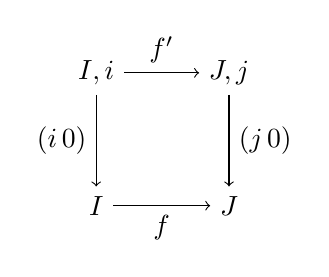
\begin{tikzpicture}[node distance=4\baselineskip]
      \node              (Ii) {$I,i$};
      \node[below of=Ii] (I)  {$I$};
      \node[right of=Ii] (Jj) {$J,j$};
      \node[below of=Jj] (J)  {$J$};

      \draw[->] (Ii) to node[left]  {$(i\,0)$} (I);
      \draw[->] (Ii) to node[above] {$f'$}     (Jj);
      \draw[->] (Jj) to node[right] {$(j\,0)$} (J);
      \draw[->] (I)  to node[below] {$f$}      (J);
    \end{tikzpicture}

    By construction $P(ρ',f')$ is a $(J,j)$-set for the extension $ρ' ∈ Γf'$ of $ρ$,
    and $af ∈ P(i\,0)(f,ρ)$ is a $J$-element.
    We define $(P \op {i} a)(f,ρ) ≔ \{ v \mid (af ,_j v) ∈ P(ρ,f')\}$.

  \item[\sc In-Pred.]
    Let $f : I,i → J$, $ρ : Γf$.  We need to define the $J$-set $(\ip {i} A P)(f,ρ)$.

    \begin{itemize}
      \item If $f$ is not defined on $i$, we have $f : I,i \stackrel{(i\,0)}{→} I \stackrel{g}{→} J$
        and we define $(\ip {i} A P)(f,ρ) ≔ A(ρ',g)$
        where $ρ' ∈ Γg$ is the restriction of $ρ ∈ Γf$.

      \item Otherwise, there is a $j ∈ J$ and $g : I → J_{\{j\}}$ such that
        the following diagram commutes

        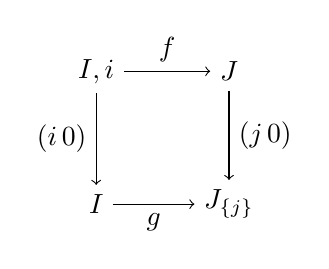
\begin{tikzpicture}[node distance=4\baselineskip]
          \node              (Ii) {$I,i$};
          \node[below of=Ii] (I)  {$I$};
          \node[right of=Ii] (J)  {$J$};
          \node[below of=J]  (Jj) {$J_{\{j\}}$};

          \draw[->] (Ii) to node[left]  {$(i\,0)$} (I);
          \draw[->] (Ii) to node[above] {$f$}      (J);
          \draw[->] (J)  to node[right] {$(j\,0)$} (Jj);
          \draw[->] (I)  to node[below] {$g$}      (Jj);
        \end{tikzpicture}

        We define $(\ip {i} A P)(f,ρ) ≔ \{ (u ,_j v) \mid u ∈ A(ρ',g), v ∈ \app{P(ρ',g)}u\}$
        where $ρ' ∈ Γg$ is the restriction of $ρ ∈ Γf$.
    \end{itemize}
\end{description}

\begin{theorem}
  If $Γ ⊢_I a : A$, $f : I → J$, $ρ ∈ Γf$, then $a(f,ρ) ∈ A(f,ρ)$.
  Furthermore $af(1,ρ) = a(f,ρ)$ (using the interpretation of
  $Γf ⊢_J af : Af$).
\end{theorem}

\begin{theorem}
  If $Γ ⊢_I a : A$ and $Γ ⊢_I b : A$ with $a = b$, then
  $a(f,ρ) = b(f,ρ)$ for any $f : I → J$ and $ρ : Γf$.
  In particular,
  \begin{itemize}
    \item $\app{λt}{u}(f,ρ) = t[u](f,ρ)$,
      where $[u]$ is the map $[u]ρ ↦ ⟨ρ,uρ⟩$, $Γ → Γ.A$
    \item $({(\ip {i} A P)} \op {i} a)(f,ρ) = (P\,a)(f,ρ)$
  \end{itemize}
\end{theorem}
\begin{proof}
  Let $f : I → J$, $i ∉ I$, $j = \fresh J$, $g : I,i → J,j$ such that
  $(i\,0)f = g(j\,0)$.
  We have
  \begin{align*}
    ({(\ip {i} A P)} \op {i} a)f
    &= \left\{ v \mid (af ,_j v) ∈ (\ip {i} A P)g \right\}
    \\
    &= \left\{ v \mid (af ,_j v) ∈ \left\{ (x ,_j y) \mid x ∈ Af, y ∈ \app{Pf} x \right\} \right\}
    \\
    &= \left\{ v \mid v ∈ \app{Pf}{af} \right\}
    \\
    &= \app{Pf}{af}
    \\
    &= \app{P}{a}f
  \qedhere
  \end{align*}
\end{proof}


\section{Related Work}

\subsection{Our own line of work}
This work continues a line of work aiming at a smooth integration of
parametricity with dependent types
\citep{bernardy_parametricity_2010,bernardy_realizability_2011,bernardy_proofs_2012,bernardy_computational_2012,bernardy_type-theory_2013}. The present work offers two improvements:
1. a denotational semantics, and
2. a much simplified syntax, suitable as the basis of a proof assistant.

The simplification of syntax is allowed by foregoing the preservation
of functions by parametricity. We call preservation of functions by
parametricity the property that if $f$ were a function, then the
canonical proof that $f$ is parametric (denoted $f \param i$ here) is
also a function. To our knowledge, all parametric \emph{models} of parametricity,
starting with \citet{reynolds_types_1983}, have this property.
However, having this property in the \emph{syntax} implies that
certain function arguments must be swapped when performing the
substitution of beta reduction, as identified by
\citet{bernardy_computational_2012}.  In the present system, the
parametric interpretation of functions is instead merely isomorphic to
a function, thanks to the {\sc In-Fun} rule (\fref{thm:iso-fun}). This
isomorphism (rather than equality) means on the one hand that the
swapping of arguments is handled by the usual rules of logic, instead
of special-purpose ones. On the other hand, obtaining the classical
parametric interpretation of types requires some purely mechanical
work by the user of the logic.

\subsection{Parametric Models of Type-Theory vs. Parametric Type-Theories}

Two pieces of work propose alternative parametric models of
type-theory
\citep{atkey_relationally_2014,krishnaswami_internalizing_2013}, but
do not integrate parametricity in the syntax of the calculus. This
means that, while certain consequences of parametricity can be made
available in the logic, via constants validated by the model,
parametricity itself is not available. In this paper, we not only
propose a parametric model, but also show how it can be used to
interpret parametricity straight up in the syntax of the type-theory.


\subsection{Various kinds of models}
Another characterising feature of proposals for parametricity is the
kind of model underlying the
semantics. \Citet{krishnaswami_internalizing_2013} propose a model
based on Q-PER. \Citet{atkey_relationally_2014} propose a model based
on reflexive graphs. The model that we use is based on cubes
(functions from subsets of colors). In
our 2012 work the cubes were reified as syntax in
an underlying calculus, while in the present work they refine a presheaf structure.

\subsection{Presheaf models}

The presheaf construction used in this paper follows a known template,
used for example by \citet{bezem2014model,DBLP:journals/corr/Pitts14}
to model univalence in type-theory.Not only both models use a
presheaf, but the underlying category is the same ($\pI$). This means
as all these models have an additional cuboidal structure.  We find
remarkable that cuboidal structures are useful for modeling both
parametricity and univalence. The present work further refines the
model by interpreting terms as $I$-elements, which is essential to
interpret our special-purpose pairing constructions.

\section{Conclusion}
\todo{We did it.}

\bibliographystyle{abbrvnat}
\bibliography{PaperTools/bibtex/jp,tt}

\end{document}
